\documentclass[11pt, letterpaper]{article}

%%% compuerta logica, funcion booleana - tipos, pulldown
%%%
%paquetes
\usepackage{tikz}
\usepackage{xcolor}
\usepackage{graphicx}
\usepackage{amsmath}
\usepackage{amssymb}
\usepackage[utf8]{inputenc} % Tildes
\usepackage[spanish]{babel} % Language
\usepackage{babelbib} % Bibliografia español
\usepackage{colortbl}
\usepackage{float}
\usepackage{fancyhdr}
\usepackage{utilidades}
\usepackage[utf8]{inputenc}
\usepackage{lastpage}
\usepackage[right = 2.5 cm, left = 2.5 cm, top = 1.5 cm , bottom = 2 cm]{geometry}
\usepackage{enumitem} %sirve para cambiar el tipo de enumeracion si redefinir comandos ejem: \arabic* \alph*
\usepackage{karnaugh-map}
\usepackage{url}
\usepackage{hyperref}

%configuraciones
\graphicspath{{img/}}
\spanishdecimal{.}	
\pagestyle{fancy}
\fancyhf{}
\renewcommand{\headrulewidth}{0pt}
\hypersetup{colorlinks=true, linkcolor=black, urlcolor=black}

%%%%%%%%%%%%%%%%%%%%%%%%%%%%%%%%%%%%%%%%%%%%%%%%%%%%%%%%%%%%%%%%%%%%%%%%%%
%%%%%%%%%%%%%%%%%%%%%%% DOCUMENT BODY %%%%%%%%%%%%%%%%%%%%%%%%%%%%%%%%%%%%
%%%%%%%%%%%%%%%%%%%%%%%%%%%%%%%%%%%%%%%%%%%%%%%%%%%%%%%%%%%%%%%%%%%%%%%%%%	

\begin{document} 
	%%%%%%%%%%%%%%%%%%%%%%%%%%%%%%%%%%%%%
	%%%%%%%%%%%%% HEADER %%%%%%%%%%%%%%%%
	%%%%%%%%%%%%%%%%%%%%%%%%%%%%%%%%%%%%%
	%%%% BLOQUE DE DATOS %%%

\newcommand{\Title}{
	Guía de Usuario para Report
} %Titulo del reporte

\newcommand{\LogoUniversity}{img/logo.jpg} %logo de la universidad
\newcommand{\NameUniversity}{Universidad Galileo} %Nombre de la universidad
\newcommand{\Date}{
	Guatemala, 6 de marzo de 2020
} %Fecha de entrega
\newcommand{\Faculty}{Facultad FISICC} %Nombre de la facultad
\newcommand{\Course}{
	Curso: *******
} %Nombre del curso
\newcommand{\ID}{
	Carnet: **** ****
}
\newcommand{\Student}{
	Alumno: Josué Benyamin Isaí Galeano Morales
} %Nombre del estudiante
\newcommand{\Section}{
	Secci\'on: *
} %Sección del estudiante
\newcommand{\Schedule}{
	Horario de laboratorio: 18:00 a 19:00
} %Horario
\newcommand{\Assistant}{
	Auxiliar: *******
} %Persona encargada
\newcommand{\Day}{
	Día de laboratorio: viernes
} %Dia en que recibe
%% FIN BLOQUE DE DATOS%%


%% NO ES NECESARIO MODIFICAR ESTA PARTE %%
\def\arraystretch{1.2}
\textbf{
	\small
	\hspace{-1 cm}
	\begin{minipage}{0.15\textwidth}
		%%%%%%%%%%%%%%%%% LOGO %%%%%%%%%%%%%%%%%%%%%%%%%%%%%%%
		\includegraphics[scale=0.5]{\LogoUniversity}
	\end{minipage}
	\begin{minipage}{0.7\textwidth}
		\resizebox{1.25\textwidth}{!}{
			\begin{tabular}{ll}
				\hline 
				%%%%% PARTE SUPERIOR DE LA TABLA DE DATOS %%%%%%%%%%%%%%%%%%%%%%%
				\NameUniversity & \Date \\
				\hline
				\rowcolor{lightgray}
				\Faculty & \Student\\
				\hline 
				\Course & \ID\\
				\hline\rowcolor{lightgray}
				\Section & \Schedule\\
				\hline 
				\Assistant & \Day\\
				\hline
			\end{tabular}
		}
	\end{minipage}
}

\vspace{0.5cm}
\begin{tikzpicture}
\hspace{-1 cm}
\draw (0.1,0.1) rectangle (1.043\textwidth,0.9);
\draw[line width=0.7mm] (0,0) rectangle (1.05\textwidth,1);
\node[font=\Large] at (0.525\textwidth, 0.45) {\textbf{\Title}};
\end{tikzpicture}		

\def\arraystretch{1}

\vspace*{0.5 cm}
 %incluimos la parte del header en el documento, note que header es como escribir dentro de un ambiente document por lo tanto no debe llevar definición de clase ni definiciones que se hagan exclusivamente en el preambulo.
		
	\begin{block}{Objetivos:}
		\begin{enumerate}
			\item Poder preparar report para usarse.
			\item Capacidad de aprovechar report.tex y sus agregados.
		\end{enumerate}
	\end{block}

	\begin{block}{Materiales:}
		\begin{enumerate}
			\item algo donde correr \LaTeX \hspace{3mm};V
			\item conexión a internet.
		\end{enumerate}
	\end{block}

	\begin{block}{Resumen:\\}
		
		En este documento se enseñara lo necesario para poder utilizar al máximo report y sus dependencias como por ejemplo Utilidades que es otro Repositorio utilizado para tener un mayor orden.
	\end{block}

	\begin{block}{Marco Teórico:\\}
		
		El repositorio \textbf{Utilidades} contiene el paquete utilidades el cual tiene algunos comandos y ambientes que pueden facilitar crear un reporte, estos pueden cambiar pero hasta el momento existen los siguientes:
		
		\begin{enumerate}
			\item \textbf{\textbackslash Center\{...\}} centra el contenido ejemplo:
			\begin{figure}[H]
				\Center{
					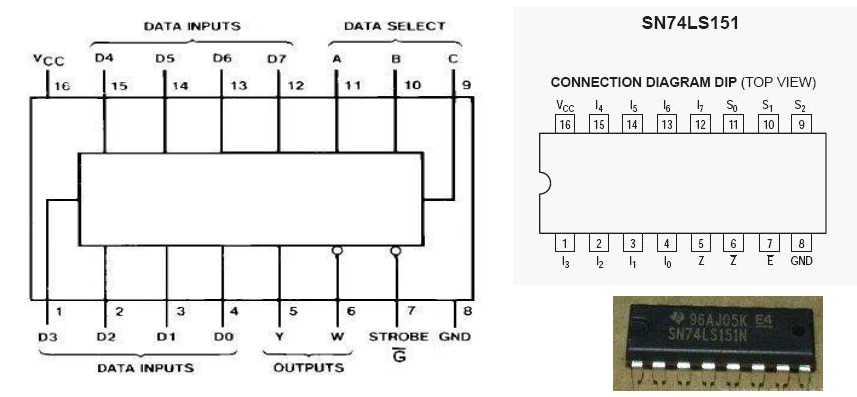
\includegraphics[scale=.6]{multiplexor}
					\caption{Información de \textbf{SN74LS151} multiplexor empleado para el laboratorio}
				}
			\end{figure}
		
			\item \textbf{\textbackslash Page[align]\{scale\}\{...\}} crea un bloque con el porcentaje dado (``scale'' que debe ser de la forma $.[$1-9$]^+$, ejemplos: .5, .3, .333, etc), align es una letra soportada por minipage ya que es un resumen del mismo por defecto es c. Ejemplo:
			
			\begin{figure}[H]
				\Page{.5}{
					\Center{
						\begin{karnaugh-map}[4][2][1][$D_1D_0$][$D_2$]
							\minterms{0,2,3,7}
							\implicant{3}{7}
							\implicantedge{0}{0}{2}{2}
						\end{karnaugh-map}
					}
					\caption{mapa de karnaugh}
				} \Page{.5}{
					\Center{
						$$\displaystyle\bar{D_2}\bar{D_0}+D_1D_0$$
					}
					\caption{Expresión}
				}
			\end{figure}
		
			\item \textbf{\textbackslash Note\{...\}} crea una nota, ejemplo:\\\\
			\Note{Esta es una nota xD la cual no se tabula y tiene un tamaño pequeño}
			
			\item \textbf{\textbackslash enumBall\{...\}} crea una bola con el contenido, ejemplo:
			
			\renewcommand{\textballcolor}{white}
			
			\Center{
				\enumBall{...}
			}
			
			\renewcommand{\ballcolor}{green}
			
			\begin{enumerate}[label=\enumBall{\arabic*}]
				\item primera bola
				\item segunda bola
			\end{enumerate}
		
			\Note{Como se puede ver las bolas pueden ser modificadas redefiniendo los comandos ballcolor y textballcolor y utilizar la combinación deseada}
			
			\item el ambiente \textbf{block} que como se puede ver se utiliza para hacer bloques en el reporte, no contiene gran cosa, pero puede ser que en el futuro se le de mayor utilidad.
			
			\item el ambiente \textbf{questions} y su comando \textbf{\textbackslash question\{...\}} son una forma de agregar preguntas y respuestas en el reporte, el ambiente recibe un argumento opcional que es el título del cuestionario por defecto es cuestionario, ejemplo:
			
			\begin{questions}[Preguntas Tontas]
				
				\question{¿Cuánto es 1+1?} la respuesta a dicha operación es $\sqrt{2}$ XD
				
				\question{¿Por qué todo junto se escribe todos separado, pero separado se escribe todo junto?} Saber we, no sé de que me hablas xs jajaja

				\question{¿Por qué escribo todo esto?} Para que sepan para que chuchas sirve cada cosa jajaja
			\end{questions}	
			 \newpage % Nueva pagina para que no se vea todo junto
			\begin{questions}
				
				\question{La pregunta} La respuesta
				
				\question{La pregunta} La respuesta
				
				\question{La pregunta} La respuesta
				
			\end{questions}
		\end{enumerate}
		
	\end{block}

	\begin{block}{Datos Prácticos:\\}
		 \begin{figure}[H]
		 	\def\arraystretch{1.5}
		 	\Center{
		 		\begin{tabular}{|c|c|c|c|}
		 			\hline
		 			\multicolumn{3}{|c|}{\textbf{Entradas}}&\multicolumn{1}{|c|}{\textbf{Salidas}}\\
		 			\hline
		 			\textbf{$D_0$}&\textbf{$D_1$}&\textbf{$D_2$}&\textbf{LED}\\
		 			\hline
		 			0 &	0 &	0 &	1\\
		 			0 &	0 &	1 &	0\\
		 			0 &	1 &	0 &	1\\
		 			0 &	1 &	1 &	1\\
		 			1 &	0 &	0 &	0\\
		 			1 &	0 &	1 &	0\\
		 			1 &	1 &	0 &	0\\
		 			1 &	1 &	1 &	1\\
		 			\hline
		 		\end{tabular}
		 	}
		 	\caption{tabla de comportamiento del LED}
		 \end{figure}
  	
  		\begin{figure}[H]
			\Page{.5}{
				\Center{
					\begin{karnaugh-map}[4][2][1][$D_1D_0$][$D_2$]
						\minterms{0,2,3,7}
						\implicant{3}{7}
						\implicantedge{0}{0}{2}{2}
					\end{karnaugh-map}
				}
				\caption{mapa de karnaugh}
			} \Page{.5}{
				\Center{
					$$\displaystyle\bar{D_2}\bar{D_0}+D_1D_0$$
				}
				\caption{Expresión}
			}
  		\end{figure}
	\end{block}

	\begin{block}{Conclusiones:\\}
		\begin{enumerate}
			\item Conclusión 1
			\item Conclusión 2
		\end{enumerate}
	\end{block}

	\bibliographystyle{apalike}
	\bibliography{referencias}
	\nocite{*}
	
\end{document}
